\documentclass{article}
\usepackage[utf8]{inputenc}

\usepackage{ifxetex}
\ifxetex
  \usepackage{fontspec}
\else
  \usepackage[T1]{fontenc}
  \usepackage[utf8]{inputenc}
  \usepackage{lmodern}
\fi

\title{Reporte de Actividad 3}
\author{Roberto Benard Orci}
\date{14/02/2018}

\begin{document}
\maketitle

\section{Introducción}
El clima es de las cosas más difíciles de predecir, existen demasiados factores que uno debe tener en consideración para hacer una buena predicción del clima. Es por eso que, con la ayuda de sondeos (con globos meteorológicos), recompilamos grandes cantidades de datos, para hacer un análisis estadístico de estos y encontrar patrones que nos sirvan para hacer predicciones cada vez más precisas.

\section{Fundamentos}

Un sondeo atmosférico es una medición de la distribución vertical de las propiedades físicas de la columna atmosférica. Tales mediciones se realizan en una variedad de formas que incluyen detección remota y observaciones. Estos normalmente se realizan con globos meteorológicos.

Un globo meteorológico, o sonoro, es un globo que transporta los instrumentos hacia arriba para recopilar información sobre diferentes propiedades físicas de la atmosfera por medio de un dispositivo de medición pequeño y reemplazable llamado radiosonda. 

Los sensores que miden los componentes atmosféricos directamente, como termómetros, barómetros y sensores de humedad, pueden ser enviados en globos, cohetes o radiosondas. También pueden transportarse en los cascos exteriores de barcos y aviones o incluso montarse en torres, ya que, lo único que se necesita para capturar las mediciones son dispositivos de almacenamiento y / o transpondedores.


\section{Análisis de datos}

Como habíamos mencionado antes, se recompilan miles y miles de datos para generar pronósticos, lo cual sería imposible de no ser por el uso de computadoras. Creamos diferentes programas de computadora que modelen diferentes propiedades con respecto a otras. En la actualidad, usamos modelos matemáticos basados en principios físicos para generar predicciones meteorológicas a corto plazo o predicciones climáticas a más largo plazo; estos últimos se aplican ampliamente para comprender y proyectar el cambio climático.

Un problema más fundamental reside en la naturaleza caótica de las ecuaciones diferenciales parciales que rigen la atmósfera. Es imposible resolver estas ecuaciones exactamente, y los pequeños errores aumentan con el tiempo (se duplican cada cinco días). La comprensión actual es que este comportamiento caótico limita los pronósticos precisos a alrededor de 14 días, incluso con datos de entrada perfectamente precisos y una falla.

\vspace{0.3cm}

En esta actividad usamos dos listas de datos de sondeos atmosféricos de la Universidad de Wyoming. Una lista de datos es del mes de diciembre y la otra de junio, a continuación, les mostraremos con el comando \textit{describe} una pequeña lista de la información "más importante" de estos archivos.

\begin{center}
	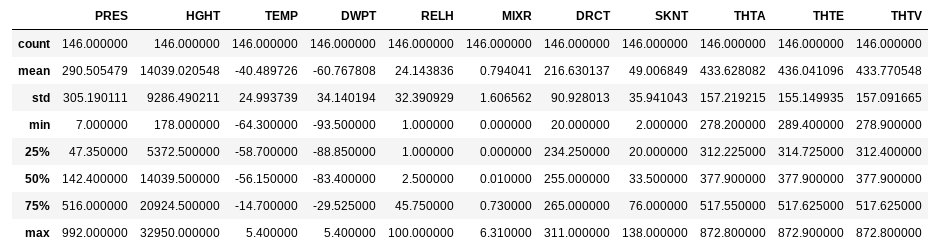
\includegraphics[width=12cm]{describeD.png}
\end{center}

\begin{center}
	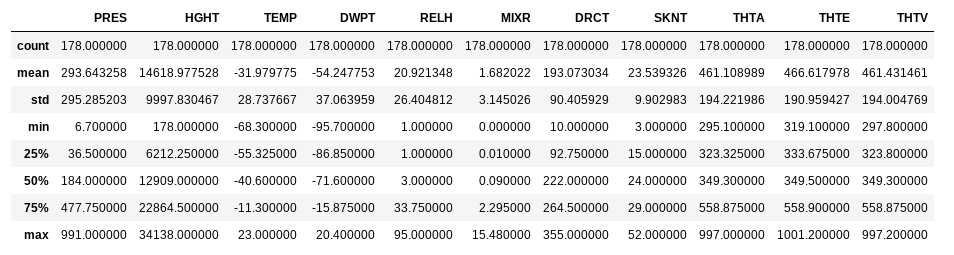
\includegraphics[width=12cm]{describeJ.png}
\end{center}

\vspace{0.3cm}

Al observar y analizar estas dos tablas de datos uno se da cuento que la mayoría de las mediciones no están distribuidas uniformemente, que los datos se inclinan para un lado, en otras palabras, que estos están bien dispersos. Es por lo que graficamos, nos da una mejor idea de lo que estamos estudiando, y de esta manera podemos sacar conclusiones.

\section{Resultados}

A continuación, mostrare las gráficas que hice junto con una breve observación para cada una.

\subsection{Variación de la presión con respecto a la altura.}

\begin{center}
	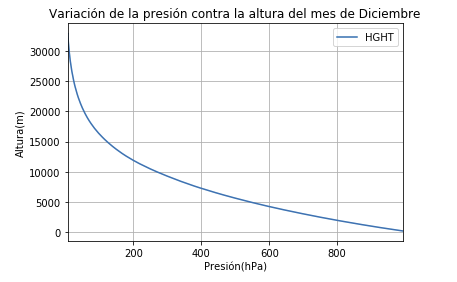
\includegraphics[width=12cm]{graph1D.png}
\end{center}

\begin{center}
	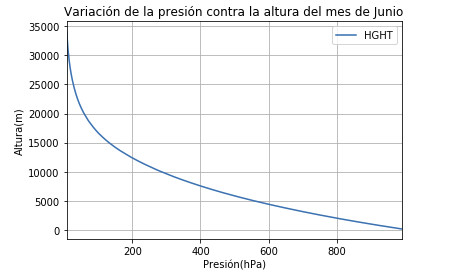
\includegraphics[width=12cm]{graph1J.png}
\end{center}
\vspace{0.3cm}

Como podemos ver en estas gráficas, la presión disminuye conforme aumenta la altura.

\subsection{Temperatura como función de la altura.}

\begin{center}
	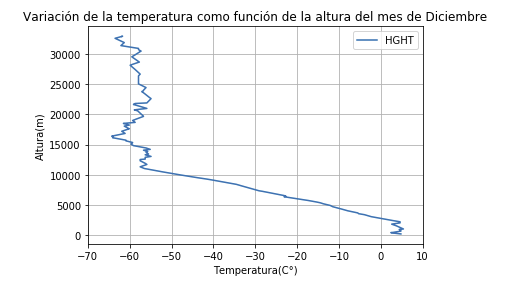
\includegraphics[width=12cm]{graph2D.png}
\end{center}

\begin{center}
	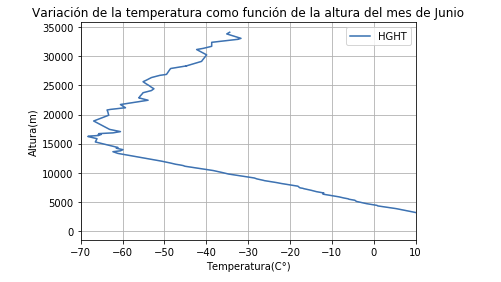
\includegraphics[width=12cm]{graph2J.png}
\end{center}
\vspace{0.3cm}

En este caso, conforme aumenta la altura la temperatura disminuye hasta un punto en donde se mantiene relativamente constante, o incluso vuelve a aumentar.

\subsection{Temperatura y temperatura de rocío como función de la altura.}

\begin{center}
	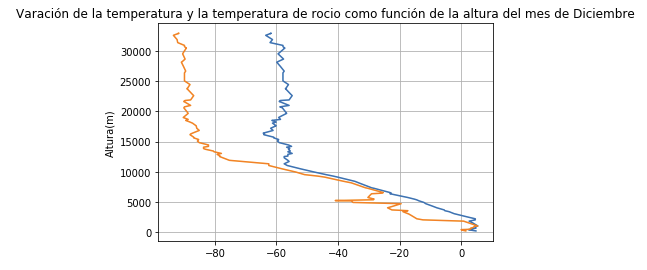
\includegraphics[width=12cm]{graph3D.png}
\end{center}

\begin{center}
	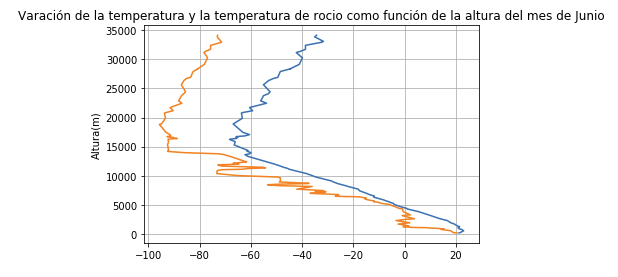
\includegraphics[width=12cm]{graph3J.png}
\end{center}
\vspace{0.3cm}

Al igual que en las gráficas pasadas, la temperatura disminuye conforme aumenta la altura hasta un punto en donde se mantiene relativamente constante o aumentan. Solo que la temperatura de rocío parece ser más propensa a cambiar por los cambios de altura.


\subsection{Rapidez de los vientos en nudos.}

\begin{center}
	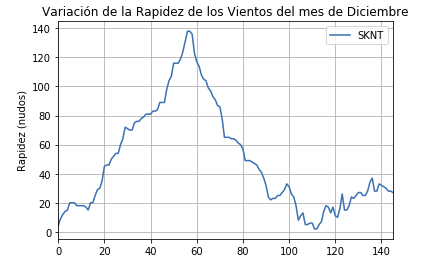
\includegraphics[width=12cm]{graph4D.png}
\end{center}

\begin{center}
	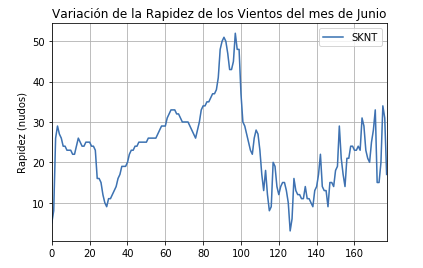
\includegraphics[width=12cm]{graph4J.png}
\end{center}
\vspace{0.3cm}

Al observar las gráficas uno llega a la conclusión de que el viento es más rápido durante el mediodía.

\subsection{Humedad relativa como función de la altura.}

\begin{center}
	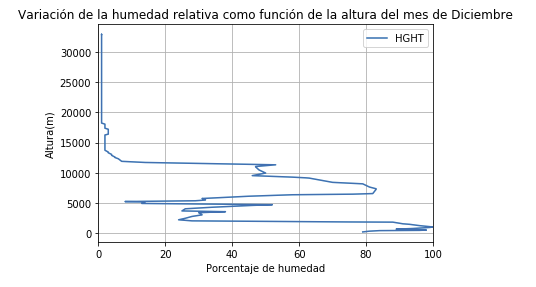
\includegraphics[width=12cm]{graph5D.png}
\end{center}

\begin{center}
	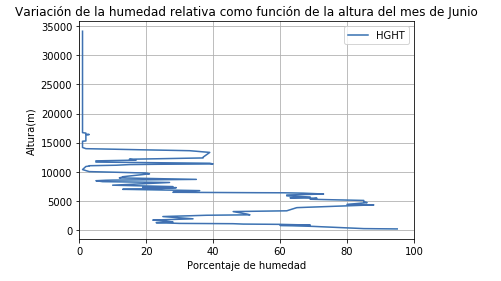
\includegraphics[width=12cm]{graph5J.png}
\end{center}
\vspace{0.3cm}

Por último, en estos dos graficas podemos observar como la humedad relativa disminuye y aumenta en un lapso muy corto al aumentar la altura, solo para volver a disminuir y legar prácticamente a 0 alrededor de los 15,000m de altura en adelante.

\section{Conclusíon}

Con el comando \textit{describe} puedes obtener información valiosa acerca de los datos que tengas, pero, aunque puedas deducir varias cosas por tu cuenta con la información que proporción esta tabla, es muy probable que pierdas parte de esta.

\vspace{0.3cm}

Por otro lado, si graficas los datos, puedes visualizar lo que pasa y darte una idea de por qué la información de la tabla es como es. En general, las gráficas serán mas fáciles de analizar y de sacar conclusiones de ellas, pero el uso de el comando y las gráficas hacen un dúo perfecto para estudiar un conjunto de datos.


\section{Bilbiografía}

\begin{verbatim}
Numerical weather prediction. (2017, October 30). Retrieved February 
12, 2018 
from https://en.wikipedia.org/wiki/Numerical_weather_
prediction#Computation 
\end{verbatim}
%https://en.wikipedia.org/wiki/Numerical_weather_prediction#Computation

\begin{verbatim}
How do I exclude a few columns from a DataFrame plot? (n.d.). Retrieved
February 12, 2018, 
from https://stackoverflow.com/questions/13003051/how-do-i-exclude-
a-few-columns-from-a-dataframe-plot
\end{verbatim}
%https://stackoverflow.com/questions/13003051/how-do-i-exclude-a-few-columns-from-a-dataframe-plot

\begin{verbatim}
Albon, C. (2017, December 20). Dropping Rows And Columns In pandas 
Dataframe. Retrieved February 12, 2018
from https://chrisalbon.com/python/data_wrangling/pandas_dropping_
column_and_rows/ 
\end{verbatim}
%https://chrisalbon.com/python/data_wrangling/pandas_dropping_column_and_rows/

\begin{verbatim}
Pandas.DataFrame.reset_index¶. (n.d.). Retrieved February 12, 2018, 
from https://pandas.pydata.org/pandas-docs/stable/generated/pandas.
DataFrame.reset_index.html 
\end{verbatim}
%https://pandas.pydata.org/pandas-docs/stable/generated/pandas.DataFrame.reset_index.html

\begin{verbatim}
Weather balloon. (2018, February 10). Retrieved February 12, 2018 
from https://en.wikipedia.org/wiki/Weather_balloon 
\end{verbatim}
%https://en.wikipedia.org/wiki/Weather_balloon

\begin{verbatim}
Changing the "tick frequency" on x or y axis in matplotlib? (n.d.). 
Retrieved February 12, 2018, 
from https://stackoverflow.com/questions/12608788/changing-the-tick
-frequency-on-x-or-y-axis-in-matplotlib
\end{verbatim}
%https://stackoverflow.com/questions/12608788/changing-the-tick-frequency-on-x-or-y-axis-in-matplotlib


\section{Apéndice}

 

    1.-¿Cuál es tu opinión general de esta actividad?
    
    \vspace{0.3cm}
    Esta práctica fue un buen ejemplo del análisis estadístico en la física, y además, del uso de herramientas computacionales (como Python) para este análisis.
    \vspace{0.3cm}
    
\noindent 2.-¿Qué fue lo que más te agradó? ¿Lo que menos te agradó?
    
    \vspace{0.3cm}
    Me gusto el poder visualizar y comparar diferentes datos de las condiciones atmosféricas para encontrar relaciones. Lo que menos me agrado fue tener que \textit{"limpiar"} los datos para eliminar cosas no deseadas de estos, pero eso no fue tanto problema.
    \vspace{0.3cm}
    
\noindent    3.-¿Que consideras que aprendiste en esta actividad? 
    
    \vspace{0.3cm}
    Como eliminar cosas no deseadas en listas de datos y nuevos comandos para visualizar mejor las gráficas.
    \vspace{0.3cm}
    
\noindent    4.-¿Qué le faltó? ¿O le sobró?   
    
    \vspace{0.3cm}
    Nada en particular, ya que se nos dice de donde sacar los datos con los que vamos a trabajar y se nos dan diferentes links para visitar y familiarizarse más con el tema, en este caso, del análisis estadístico del clima.
    \vspace{0.3cm}
    
\noindent    5.-¿Que mejoras sugieres a la actividad?
    
    \vspace{0.3cm}
    Siento que, en general, sería bueno dar media hora a la semana (al inicio de una práctica) para hablar de las nuevas herramientas que se nos espera aprender.
    \vspace{0.3cm}
    

\end{document}